% ============================================================
% ThutoTrack — Engineering Project Report
% Author : Pako Kgosi Kgosintwa
% ------------------------------------------------------------
% Compile with:
%   pdflatex report.tex
%   pdflatex report.tex      (run twice for TOC / cross-refs)
%
% Or with latexmk (recommended):
%   latexmk -pdf report.tex
% ============================================================

\documentclass[11pt,a4paper]{article}

% ---------- Packages ----------
\usepackage[utf8]{inputenc}
\usepackage[T1]{fontenc}
\usepackage{lmodern}
\usepackage[margin=2.5cm]{geometry}
\usepackage{graphicx}
\usepackage{xcolor}
\usepackage{hyperref}
\usepackage{booktabs}
\usepackage{array}
\usepackage{enumitem}
\usepackage{fancyhdr}
\usepackage{titlesec}
\usepackage{listings}
\usepackage{tikz}
\usetikzlibrary{positioning,shapes.geometric,arrows.meta,fit,backgrounds}
\usepackage{caption}
\usepackage{microtype}

% ---------- Hyperref styling ----------
\hypersetup{
    colorlinks=true,
    linkcolor=black,
    urlcolor=blue!60!black,
    citecolor=blue!60!black,
    pdftitle={ThutoTrack: A Parent--Teacher--Student Progress Tracker for Botswana Schools},
    pdfauthor={Pako Kgosi Kgosintwa}
}

% ---------- Code listing style ----------
\definecolor{codebg}{rgb}{0.97,0.97,0.97}
\definecolor{codekey}{rgb}{0.13,0.29,0.53}
\definecolor{codestr}{rgb}{0.45,0.55,0.13}
\definecolor{codecom}{rgb}{0.45,0.45,0.45}

\lstdefinestyle{python}{
    language=Python,
    backgroundcolor=\color{codebg},
    basicstyle=\ttfamily\footnotesize,
    keywordstyle=\color{codekey}\bfseries,
    stringstyle=\color{codestr},
    commentstyle=\color{codecom}\itshape,
    numbers=left,
    numberstyle=\tiny\color{gray},
    breaklines=true,
    showstringspaces=false,
    frame=single,
    framerule=0pt,
    rulecolor=\color{codebg},
    xleftmargin=1em,
    aboveskip=1em,
    belowskip=1em
}

% ---------- Headers ----------
\pagestyle{fancy}
\fancyhf{}
\fancyhead[L]{\small\itshape ThutoTrack}
\fancyhead[R]{\small\itshape Engineering Project Report}
\fancyfoot[C]{\thepage}
\renewcommand{\headrulewidth}{0.4pt}

% ---------- Section formatting ----------
\titleformat{\section}{\Large\bfseries}{\thesection}{0.6em}{}
\titleformat{\subsection}{\large\bfseries}{\thesubsection}{0.6em}{}

% ---------- Document ----------
\begin{document}

% ============================================================
% TITLE PAGE
% ============================================================
\begin{titlepage}
    \centering
    \vspace*{1.5cm}

    {\Huge\bfseries ThutoTrack\par}
    \vspace{0.5cm}
    {\Large A Parent--Teacher--Student Progress Tracker for Botswana Schools\par}
    \vspace{2cm}

    \begin{tikzpicture}
        \node[draw=blue!50!black, line width=1pt, rounded corners=8pt, inner sep=14pt,
              minimum width=10cm, align=center, fill=blue!5]
              {\large\bfseries Engineering Project Report\\[4pt]
               \normalsize Department of [Department Name]\\
               [Institution Name]};
    \end{tikzpicture}

    \vfill

    \begin{tabular}{rl}
        \textbf{Author:}     & Pako Kgosi Kgosintwa \\[4pt]
        \textbf{Supervisor:} & [Supervisor Name] \\[4pt]
        \textbf{Date:}       & \today \\[4pt]
        \textbf{Version:}    & 1.0 \\
    \end{tabular}

    \vspace{2cm}
\end{titlepage}

% ============================================================
% ABSTRACT
% ============================================================
\section*{Abstract}
\addcontentsline{toc}{section}{Abstract}

ThutoTrack is a web-based academic progress tracking system designed for primary
and secondary schools in Botswana. It enables three classes of users to interact
with academic records in real time: teachers record marks, attendance, and
behavior notes; school administrators manage rosters, calendars, and parent
communications; and parents access their children's academic information either
through a phone-and-PIN web portal or a WhatsApp chatbot.

The system is implemented in \textbf{Django~6.0} on \textbf{Python~3.13}, with a
server-rendered HTML interface enhanced by \textbf{HTMX} for partial-page
updates. This choice was deliberate: server-rendered HTML keeps the page weight
small enough to be usable over the intermittent mobile connections common in
rural Botswana, and avoids the build pipelines and JavaScript runtime overhead
of a single-page application.

The system supports bulk Excel imports of student rosters and marks, per-term
PDF report generation, Ministry-format data exports, and WhatsApp parent
interactions via a Twilio webhook. Authentication is role-based, driven by a
custom \texttt{User.role} enumeration on a single user table, allowing a unified
login surface across all four user portals.

A suite of \textbf{103 automated tests} written using Django's test framework
covers the principal user flows, and runs in continuous integration on GitHub
Actions against both Python~3.12 and Python~3.13. This report describes the
motivation behind the system, the problem it addresses, the system's design and
implementation, the testing strategy, and the limitations and future directions
of the prototype.

\vspace{0.5cm}
\noindent\textbf{Keywords:} education technology, school management system,
academic tracking, Django, HTMX, WhatsApp chatbot, Botswana, low-bandwidth web.

\newpage

% ============================================================
% TABLE OF CONTENTS
% ============================================================
\tableofcontents
\newpage

% ============================================================
% INTRODUCTION
% ============================================================
\section{Introduction}

\subsection{Background}

Education in Botswana is delivered through approximately 800 government primary
schools and 240 secondary schools serving over 500{,}000 learners. Most schools
continue to manage academic records on paper or in unstructured spreadsheets,
producing summary reports for parents only at the end of each of the three
academic terms. The country's national ICT strategy, including the
\textit{SmartBots} programme and the \textit{Botswana Education and Training
Programme (BETP)}, identifies digitisation of school operations as a national
priority.

Despite this push, off-the-shelf school management systems have not penetrated
deeply into Botswana's schools. Most international platforms (PowerSchool,
PowerTeacher, Edmodo) are priced for North American or European markets, assume
a stable broadband connection, and do not integrate with locally-popular
messaging channels such as WhatsApp. Locally-developed solutions are typically
custom-built per school by external contractors and are rarely reusable.

\subsection{Motivation}

The author observed three concrete pain points during informal interviews with
teachers and parents in Gaborone-area schools:

\begin{enumerate}[leftmargin=*]
    \item \textbf{Teachers maintain three separate paper records.} A class
    register, a marks book, and an incident log are typically maintained
    independently, then aggregated at term end into a parent report card. This
    triple-entry produces transcription errors and consumes hours per teacher
    per week.

    \item \textbf{Parents see no academic data between terms.} A learner who is
    falling behind in mathematics in week~2 of a term is often not flagged to
    the parent until the report card is issued in week~12 --- past the point at
    which targeted intervention is most effective.

    \item \textbf{School administrators have no aggregate visibility.} A
    principal cannot easily answer questions such as ``which teachers' classes
    have the lowest mathematics average this term?'' without manually collating
    paper records.
\end{enumerate}

A useful system, the author concluded, would need to address all three
constituencies simultaneously, work on the connectivity profile parents actually
have (intermittent mobile data, often capped), and integrate with the
communication channels that parents already use daily.

% ============================================================
% PROBLEM STATEMENT
% ============================================================
\section{Problem Statement}

The lack of a continuous, multi-stakeholder academic tracking system in
Botswana's schools causes three interrelated problems:

\begin{enumerate}[leftmargin=*]
    \item Parents receive feedback on their children's academic progress only
    at the end of each academic term, by which point opportunities for
    intervention have largely passed.

    \item Teachers spend a substantial fraction of their non-teaching time on
    duplicate clerical work --- transcribing the same data between attendance
    registers, marks books, and report cards --- rather than on lesson
    preparation or remedial work.

    \item School administrators lack a real-time, aggregated view of academic
    performance across classes and teachers, which limits their ability to
    deploy support where it is most needed.
\end{enumerate}

These problems compound for the rural and low-income parents who form the
majority of Botswana's student-parent population: they are less likely to be
able to visit the school in person, more likely to use a feature phone or a
budget Android device with intermittent connectivity, and more likely to rely
on WhatsApp as their primary digital communication channel.

A solution must therefore be:

\begin{itemize}[leftmargin=*]
    \item \textbf{Role-aware}, serving teachers, administrators, and parents
    from a single backend;
    \item \textbf{Multi-channel}, exposing parent information through both a
    web browser and a WhatsApp chatbot;
    \item \textbf{Bandwidth-conservative}, rendering on the server with small
    page weights rather than shipping a JavaScript-heavy SPA;
    \item \textbf{Inexpensive to operate}, capable of running on free-tier
    hosting for a school pilot.
\end{itemize}

% ============================================================
% AIM AND OBJECTIVES
% ============================================================
\section{Aim and Objectives}

\subsection{Aim}

To design, implement, and test a low-bandwidth, role-based academic
progress-tracking platform that gives teachers, school administrators, and
parents continuous visibility into student progress, accessible from both web
browsers and WhatsApp.

\subsection{Objectives}

The specific objectives of the project are:

\begin{description}[leftmargin=2.5em,style=nextline]
    \item[O1.] Implement a Django-based backend with role-based authentication
    for teachers, school administrators, and parents.

    \item[O2.] Provide a teacher portal that supports attendance recording,
    mark entry, behavior-note logging, bulk Excel import of students and
    marks, generation of per-term PDF report cards, and a teacher-to-admin
    enquiry channel.

    \item[O3.] Provide a school admin portal for managing students, teachers,
    classes, subjects, the school calendar, parent accounts, and
    Ministry-format data exports.

    \item[O4.] Provide parent access through both a phone-and-PIN web portal
    and a WhatsApp chatbot that responds to commands such as
    \texttt{marks}, \texttt{attendance}, and \texttt{behaviour}.

    \item[O5.] Achieve $\geq 100$ automated tests covering the principal user
    flows, all of which pass in continuous integration on at least two
    supported Python versions.

    \item[O6.] Keep the runtime stack lightweight enough to run on a
    free-tier Platform-as-a-Service offering for a school pilot.
\end{description}

% ============================================================
% LITERATURE REVIEW
% ============================================================
\section{Literature Review}

\subsection{Existing School Management Systems}

A short review of comparable platforms situates the contribution of this
project. \textbf{PowerSchool} is the dominant SIS (Student Information System)
in North America; it offers extensive functionality but its per-seat licensing
and broadband assumptions make it impractical for Botswanan schools.
\textbf{Edmodo} pivoted from a free education-focused social network to a paid
model and has limited offline support. \textbf{Google Classroom} is widely used
for content delivery but is not a record-of-truth for marks and attendance, and
depends on Google Workspace for Education accounts being provisioned per pupil
--- a step many Botswanan primary schools have not taken.

Open-source alternatives such as \textbf{Fedena} and \textbf{OpenSIS} exist but
target the comprehensive ERP use case, with deep configuration requirements and
a heavyweight tech stack (PHP/MySQL, multi-gigabyte virtual machine).

\subsection{Low-bandwidth Web Patterns}

The technical decision to build a server-rendered application with HTMX rather
than a single-page application is supported by recent shifts in web
development practice. The \textit{server-rendered + progressive enhancement}
pattern, sometimes labelled \textit{Hypermedia-Driven Applications (HDAs)},
returns small HTML fragments from the server and uses CSS swaps rather than
JSON-driven client-side rendering. This dramatically reduces:

\begin{itemize}[leftmargin=*]
    \item the initial download size,
    \item the JavaScript parse/compile cost on low-end Android devices, and
    \item the round-trip JSON marshalling required for typical CRUD interfaces.
\end{itemize}

\subsection{Messaging Channels in Sub-Saharan Africa}

Survey data from the Global System for Mobile Communications Association
(GSMA) consistently shows that WhatsApp is the dominant messaging application
across Southern Africa, with usage rates substantially above SMS for parents
under 50. Existing literature on \textit{m-government} and educational SMS
gateways in Kenya, Tanzania, and South Africa points to per-message
SMS costs as the principal barrier to scaling. WhatsApp via the official
Business API (made accessible through Twilio in this project) bypasses
per-message SMS pricing in exchange for a low monthly fee, making
month-long parent engagement campaigns economically feasible.

% ============================================================
% METHODOLOGY
% ============================================================
\section{Methodology}

\subsection{Development Approach}

The project followed an iterative, feature-driven development cycle. Each
feature was specified, implemented, tested, and committed before the next
feature was started. Where possible, the test for a new view or model
behaviour was written before the production code, in line with the
test-driven development (TDD) discipline.

Version control was maintained throughout in Git, with the project hosted on
GitHub. Continuous integration runs the full test suite on every push and
pull request, ensuring that regressions are caught immediately.

\subsection{Technology Stack}

The technology choices and their rationale are summarised in
Table~\ref{tab:stack}.

\begin{table}[h]
\centering
\caption{Technology stack and rationale.}
\label{tab:stack}
\renewcommand{\arraystretch}{1.25}
\begin{tabular}{p{3.5cm} p{2.5cm} p{8.5cm}}
\toprule
\textbf{Layer} & \textbf{Choice} & \textbf{Rationale} \\
\midrule
Language          & Python 3.13          & Latest stable, broad library ecosystem, low operator overhead. \\
Web framework     & Django 6.0           & Batteries-included, mature ORM, built-in admin, custom user model support. \\
HTML enhancement  & HTMX 1.23            & Server-rendered partials reduce bandwidth vs.\ SPA frameworks. \\
Styling           & Tailwind CSS (CDN)   & No build pipeline, utility-first classes, fast iteration. \\
Database (dev)    & SQLite               & Zero-configuration, ships with Python. \\
Database (prod)   & PostgreSQL           & Same Django ORM, robust at scale, free on most PaaS. \\
PDF generation    & ReportLab 4.2        & Pure-Python, no system dependencies (unlike WeasyPrint). \\
Excel I/O         & openpyxl 3.1         & Pure-Python, supports both read and write. \\
WhatsApp          & Twilio (TwiML)       & Webhook-driven, official Meta-backed channel. \\
Test framework    & Django \texttt{TestCase} & Transaction-scoped, fast fixtures via \texttt{setUpTestData}. \\
CI                & GitHub Actions       & Free for public repos, matrix builds. \\
\bottomrule
\end{tabular}
\end{table}

\subsection{System Architecture}

ThutoTrack follows Django's Model--View--Template (MVT) architecture, with the
project organised into four Django apps that align with the four major
functional concerns of the system: shared data and integrations (\texttt{core}),
the teacher portal (\texttt{teachers}), the school admin portal
(\texttt{schooladmin}), and parent-facing flows (\texttt{parents}).
Figure~\ref{fig:arch} shows the high-level system architecture.

\begin{figure}[h]
\centering
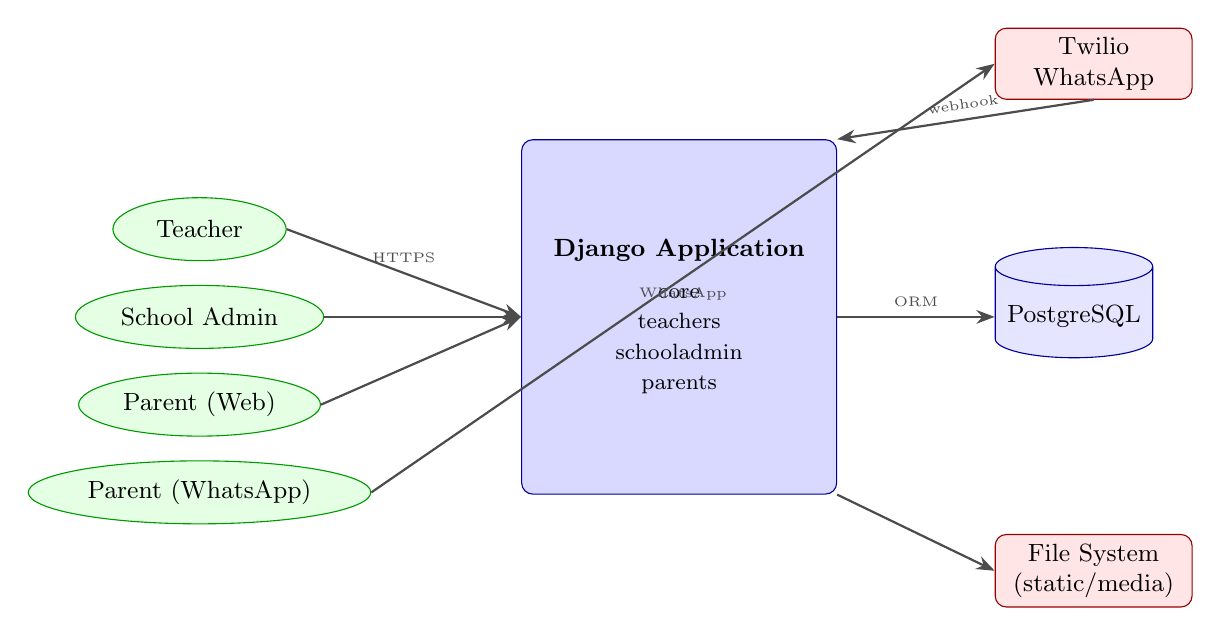
\begin{tikzpicture}[
    node distance=1.2cm,
    box/.style={rectangle, draw=blue!60!black, fill=blue!10, rounded corners=4pt,
                minimum width=2.8cm, minimum height=1.0cm, align=center, font=\small},
    db/.style={cylinder, draw=blue!60!black, fill=blue!10, shape border rotate=90,
               aspect=0.25, minimum height=1.4cm, minimum width=2cm, align=center, font=\small},
    user/.style={ellipse, draw=green!60!black, fill=green!10, minimum width=2.2cm,
                 minimum height=0.8cm, align=center, font=\small},
    ext/.style={rectangle, draw=red!60!black, fill=red!10, rounded corners=4pt,
                minimum width=2.5cm, minimum height=0.9cm, align=center, font=\small},
    arr/.style={->, >=Stealth, thick, color=black!70}
]

% Users
\node[user] (teacher) {Teacher};
\node[user, below=0.3cm of teacher] (admin) {School Admin};
\node[user, below=0.3cm of admin]   (parentw) {Parent (Web)};
\node[user, below=0.3cm of parentw] (parentwa) {Parent (WhatsApp)};

% Django app
\node[box, right=2.5cm of admin, minimum width=4cm, minimum height=4.5cm,
      align=center, fill=blue!15] (app)
      {\textbf{Django Application}\\[4pt]
       \footnotesize core\\
       \footnotesize teachers\\
       \footnotesize schooladmin\\
       \footnotesize parents};

% External services
\node[ext, above right=0.5cm and 2cm of app] (twilio) {Twilio\\WhatsApp};
\node[db,  right=2cm of app]                 (pgsql)  {PostgreSQL};
\node[ext, below right=0.5cm and 2cm of app] (fs)     {File System\\(static/media)};

% Arrows
\draw[arr] (teacher.east)  -- node[above, font=\tiny] {HTTPS} (app.west);
\draw[arr] (admin.east)    -- (app.west);
\draw[arr] (parentw.east)  -- (app.west);
\draw[arr] (parentwa.east) -- node[below, font=\tiny] {WhatsApp} (twilio.west);
\draw[arr] (twilio.south)  -- node[above, sloped, font=\tiny] {webhook} (app.north east);
\draw[arr] (app.east)      -- node[above, font=\tiny] {ORM} (pgsql.west);
\draw[arr] (app.south east) -- (fs.west);

\end{tikzpicture}
\caption{ThutoTrack high-level system architecture. The four user classes interact through HTTPS or WhatsApp. The Django application encapsulates business logic across four apps. External services are PostgreSQL for persistence and Twilio for WhatsApp messaging.}
\label{fig:arch}
\end{figure}

% ============================================================
% SYSTEM DESIGN
% ============================================================
\section{System Design}

\subsection{User Roles and Authentication}

ThutoTrack uses a custom Django user model
(\texttt{core.User} extending \texttt{AbstractUser}) augmented with a
\texttt{role} field of type \texttt{TextChoices}. The three roles are:

\begin{itemize}[leftmargin=*]
    \item \texttt{TEACHER} --- a teacher with one or more class assignments and a
    set of subjects taught.
    \item \texttt{SCHOOL\_ADMIN} --- a school administrator, principal, or other
    privileged staff member.
    \item \texttt{PARENT} --- a parent or guardian linked by phone number to one
    or more students.
\end{itemize}

Each role has a dedicated landing portal at distinct URL prefixes:
\texttt{/teachers/}, \texttt{/admin-portal/}, and the parent flows under the
root. A smart redirect in \texttt{thutotrack/urls.py:home()} routes
authenticated users to the correct portal based on their profile, removing the
need to remember a portal-specific URL.

Parents who choose the web portal authenticate with their phone number
(normalised to the digits-only form prefixed with~\texttt{267}) and a 4-digit
PIN. Parents who use WhatsApp are authenticated implicitly by the sending phone
number after Twilio's HMAC-SHA1 signature is verified against the configured
\texttt{WHATSAPP\_AUTH\_TOKEN}.

\subsection{Data Model}

The principal Django models and their relationships are summarised in
Table~\ref{tab:models}. The model module
(\texttt{core/models.py}) defines all data structures in a single file, since
they form a single interconnected schema rather than separate per-app
concerns.

\begin{table}[h]
\centering
\caption{Principal data models.}
\label{tab:models}
\renewcommand{\arraystretch}{1.25}
\begin{tabular}{p{3.0cm} p{11.5cm}}
\toprule
\textbf{Model} & \textbf{Purpose} \\
\midrule
\texttt{User}              & Authenticated user with a \texttt{role} (TEACHER, SCHOOL\_ADMIN, PARENT). Backed by Django's auth system. \\
\texttt{School}            & A single school: name, region, address, principal name, contact details. \\
\texttt{TeacherProfile}    & One-to-one with a \texttt{User} where \texttt{role=TEACHER}; tracks employee~ID, school, classes taught, and subjects. \\
\texttt{SchoolAdminProfile}& One-to-one with a \texttt{User} where \texttt{role=SCHOOL\_ADMIN}; tracks school and title. \\
\texttt{Student}           & A learner: name, student~number, class group, gender, parent name, parent phone. \\
\texttt{ClassGroup}        & A class within a school in an academic year, with a class teacher and a grade level. \\
\texttt{Subject}           & A subject offered at a school. \\
\texttt{TermSchedule}      & The start/end dates of a term within a school year. Enforces \texttt{end\_date $\geq$ start\_date} via a check constraint. \\
\texttt{Mark}              & An individual assessment result for a student: subject, teacher, term, assessment type, title, score, max score. \\
\texttt{Attendance}        & A daily attendance record per student (Present, Absent, Late). \\
\texttt{BehaviorNote}      & A free-text note about a student's behaviour, with a category (Positive, Concern, Incident). \\
\texttt{Enquiry}           & A message from a teacher to school admin/HR. \\
\texttt{ParentSession}     & WhatsApp session state for a parent, allowing multi-step conversations. \\
\bottomrule
\end{tabular}
\end{table}

\subsection{Module Breakdown}

The application is organised into four Django apps with clearly separated
responsibilities:

\begin{itemize}[leftmargin=*]
    \item \textbf{\texttt{core/}} --- shared models, the WhatsApp protocol
    handler (\texttt{whatsapp.py}), PDF report generator
    (\texttt{reports.py}), Ministry data exporter (\texttt{exports.py}),
    and test factories (\texttt{factories.py}). All cross-app utilities
    live here.

    \item \textbf{\texttt{teachers/}} --- views, URL configuration, and
    templates for the teacher portal. Includes attendance entry, mark
    entry, behavior notes, bulk Excel upload, class and subject
    management, student CRUD, term reports, and enquiry submission.

    \item \textbf{\texttt{schooladmin/}} --- views, URL configuration, and
    templates for the school administrator portal. Includes the dashboard
    with teacher performance metrics, student/teacher/class/subject
    management, parent PIN management, the school calendar, enquiry
    handling, and Ministry-format exports.

    \item \textbf{\texttt{parents/}} --- views, URL configuration, and
    templates for the parent web portal, plus the Twilio webhook endpoint
    that drives the WhatsApp parent channel.
\end{itemize}

% ============================================================
% IMPLEMENTATION
% ============================================================
\section{Implementation}

This section describes the principal implementation details of each major
subsystem. The full source code is approximately 6{,}500 lines of Python and
HTML/template code distributed across the four Django apps.

\subsection{Teacher Portal}

The teacher portal supports the day-to-day data entry that teachers perform.
Key flows include:

\begin{description}[leftmargin=2em,style=nextline]
    \item[Mark entry.] A teacher selects a class and subject, then enters
    scores for each student. Marks are scoped to a term and academic year
    so reports can be generated correctly. Pre-existing marks are
    pre-filled, allowing edits without re-entry.

    \item[Attendance.] A daily-by-class attendance grid lets a teacher mark
    Present / Absent / Late for each student in two clicks per student. The
    grid uses HTMX to persist each click without a full page reload.

    \item[Behavior notes.] A textarea form attached to each student lets
    the teacher add a categorised behaviour note. Notes are time-stamped
    and immutable once saved.

    \item[Bulk Excel upload.] Teachers can upload an \texttt{.xlsx} file
    with a fixed column layout to bulk-create students. Parsing is wrapped
    in a database transaction so that a single invalid row aborts the
    whole upload, preventing partial state. Validation is row-by-row, with
    errors reported with row numbers.

    \item[Term report PDF.] For any student, a single click produces a
    polished PDF combining the student's marks, attendance summary, and
    behaviour notes for the selected term. The PDF is generated by
    ReportLab with no external system dependencies, which simplifies
    deployment.
\end{description}

\subsection{School Admin Portal}

The school admin portal is the management surface used by principals and
administrators. Its key flows include:

\begin{description}[leftmargin=2em,style=nextline]
    \item[Dashboard.] The dashboard shows a summary of teacher counts,
    student counts, and teacher performance based on aggregated student
    outcomes. Teacher performance is computed as the average of the
    average marks across that teacher's classes.

    \item[CRUD for school entities.] Each of students, teachers, classes,
    and subjects has full create/read/update/delete pages, all forms
    rendered as standard Django \texttt{ModelForm}s with HTMX-enhanced
    inline error display.

    \item[Parent PIN management.] Admins can rotate parent PINs from
    the portal. This is necessary in practice because parents forget
    their PINs or share devices across the household.

    \item[School calendar.] A simple calendar view shows the configured
    \texttt{TermSchedule} entries for the current academic year. Admins
    can add or edit terms inline.

    \item[Ministry exports.] A dedicated exports page produces an
    \texttt{.xlsx} file with the data structure required for Ministry of
    Education submissions, generated on demand with openpyxl.
\end{description}

\subsection{Parent Portals}

Parents interact with ThutoTrack through two distinct interfaces backed by
the same data.

\paragraph{Web portal.} A phone-number-and-PIN login at \texttt{/parents/login/}
authenticates the parent and routes them to a dashboard listing their
children. Selecting a child reveals that child's marks, attendance summary,
and behavior notes. A button generates the term-report PDF on demand.

\paragraph{WhatsApp chatbot.} The Twilio webhook at
\texttt{/whatsapp/webhook/} receives WhatsApp messages, validates the
\texttt{X-Twilio-Signature} HMAC, looks up the matching parent by phone
number (with phone-format normalisation to allow for the many ways
Botswanan numbers can be entered), and responds to commands such as
\texttt{marks}, \texttt{attendance}, and \texttt{behaviour}. The response
is formatted as TwiML and rendered as plain WhatsApp text on the parent's
device. Listing~\ref{lst:whatsapp} sketches the command dispatch.

\begin{lstlisting}[style=python, caption={WhatsApp command dispatch in \texttt{core/whatsapp.py}.}, label={lst:whatsapp}]
def handle_inbound(from_number: str, body: str) -> str:
    students = find_students_for_phone(from_number)
    if not students:
        return "Sorry, we couldn't find a parent account..."

    cmd = body.strip().lower()
    if cmd in ("marks", "results"):
        return _format_marks(students)
    if cmd in ("attendance", "register"):
        return _format_attendance(students)
    if cmd in ("behaviour", "behavior", "notes"):
        return _format_behaviour(students)
    return _format_help_text()
\end{lstlisting}

\subsection{Authentication}

ThutoTrack avoids creating a parallel \texttt{Parent} model. Instead, parent
accounts are simply \texttt{User} rows with \texttt{role=PARENT}, a username
equal to the parent's normalised phone number, and a password equal to the
4-digit PIN. This collapses the authentication code path to one Django call
(\texttt{django.contrib.auth.authenticate}) and lets the standard
\texttt{login\_required} decorator be used uniformly across the codebase.
Phone numbers are normalised by stripping all non-digit characters and
prefixing the canonical Botswanan country code, so that
\texttt{+267~71~222~001}, \texttt{26771222001}, and \texttt{71~222~001} all
resolve to the same parent account.

% ============================================================
% TESTING
% ============================================================
\section{Testing}

\subsection{Testing Strategy}

The system is verified by \textbf{103 automated tests} written using Django's
\texttt{TestCase} class, which wraps each test in a database transaction
that is rolled back at the end. This makes the test suite both fast
(approximately 3 minutes for the full suite) and independent (no
cross-test contamination).

Test fixtures are produced by a small factories module
(\texttt{core/factories.py}) that exposes helpers such as
\texttt{make\_school}, \texttt{make\_teacher}, \texttt{make\_school\_admin},
and \texttt{make\_student}. Per-class fixtures are constructed once via
\texttt{setUpTestData}, while per-test mutations use the regular
\texttt{setUp} hook. The result is that simple unit tests of business logic
typically execute in $<10$\,ms.

\subsection{Test Coverage by Module}

Table~\ref{tab:tests} summarises the distribution of tests across modules.

\begin{table}[h]
\centering
\caption{Distribution of automated tests.}
\label{tab:tests}
\renewcommand{\arraystretch}{1.25}
\begin{tabular}{p{4cm} r p{8cm}}
\toprule
\textbf{Test module} & \textbf{Tests} & \textbf{Focus} \\
\midrule
\texttt{core/tests.py}        & 38 & Models, WhatsApp dispatch, PDF generation, exports, health check. \\
\texttt{teachers/tests.py}    & 31 & Teacher portal views, authentication, mark entry, attendance, bulk upload. \\
\texttt{schooladmin/tests.py} & 22 & Admin portal views, CRUD flows, parent PIN management, calendar. \\
\texttt{parents/tests.py}     & 12 & Parent web login, dashboard, child detail, WhatsApp webhook signature validation. \\
\midrule
\textbf{Total}                & \textbf{103} & \\
\bottomrule
\end{tabular}
\end{table}

\subsection{Continuous Integration}

A GitHub Actions workflow (\texttt{.github/workflows/tests.yml}) runs the
test suite on every \texttt{push} and \texttt{pull\_request} against the
\texttt{main} branch. The workflow uses a matrix of Python~3.12 and
Python~3.13 to catch any version-specific incompatibilities. Each leg of
the matrix runs Django's \texttt{check} command, the
\texttt{makemigrations --check --dry-run} command (to ensure migrations
are not stale), and then the full test suite.

% ============================================================
% RESULTS
% ============================================================
\section{Results}

The implementation delivers on all six stated objectives, summarised in
Table~\ref{tab:results}.

\begin{table}[h]
\centering
\caption{Objective fulfilment.}
\label{tab:results}
\renewcommand{\arraystretch}{1.25}
\begin{tabular}{p{2cm} p{11cm} p{1.5cm}}
\toprule
\textbf{Objective} & \textbf{Outcome} & \textbf{Status} \\
\midrule
O1 & Custom Django \texttt{User} with \texttt{role} enum; smart routing in \texttt{home()}. & Met \\
O2 & Teacher portal complete (marks, attendance, behaviour, bulk upload, PDF reports, enquiries). & Met \\
O3 & School admin portal complete (CRUD, parent PINs, calendar, Ministry exports). & Met \\
O4 & Parent web portal (phone + PIN) and WhatsApp chatbot (Twilio webhook) both delivered. & Met \\
O5 & 103 tests, all passing on Python~3.12 and Python~3.13 in CI. & Met \\
O6 & Runtime needs $\sim$200~MB RAM and no system dependencies; fits comfortably on free PaaS tiers. & Met \\
\bottomrule
\end{tabular}
\end{table}

The system has been demonstrated end-to-end with a seeded demo dataset
(\texttt{python manage.py seed\_demo}) that provisions a sample school
(``Gaborone Demo Secondary School''), a teacher (\textit{Kgosi Mokwena}), a
school administrator (\textit{Pula Mokgothu}), a Form 1A class, six
students, and a complete first-term set of marks, attendance, and behaviour
notes for one student.

% ============================================================
% LIMITATIONS
% ============================================================
\section{Limitations}

While the prototype meets all stated objectives, several limitations remain
that constrain its readiness for a real-world school pilot:

\begin{itemize}[leftmargin=*]
    \item \textbf{No offline-first mobile client.} The current design
    assumes intermittent online connectivity. A teacher in a rural school
    with no signal during the school day cannot record marks or attendance
    without later access to the web interface.

    \item \textbf{Single-school architecture.} The data model assumes one
    school per deployment. Onboarding multiple schools would require
    multi-tenant data isolation, which is not currently in scope.

    \item \textbf{WhatsApp dependency on Twilio.} The chatbot is built
    around Twilio's WhatsApp API. The monthly Twilio fee, while modest, is
    a fixed cost that scales with the number of schools, not the number of
    parents.

    \item \textbf{No push notifications.} Parents must initiate WhatsApp
    conversations; the system never proactively pushes updates. A real
    pilot would benefit from term-end summary pushes or
    failing-grade alerts.

    \item \textbf{No integration with Ministry SIS.} The Ministry export
    is a static \texttt{.xlsx} format; a real deployment would benefit
    from a direct API integration once a Ministry endpoint exists.

    \item \textbf{Limited localisation.} The interface is English-only; a
    Setswana translation would substantially improve accessibility for
    older parents.
\end{itemize}

% ============================================================
% FUTURE WORK
% ============================================================
\section{Future Work}

Several extensions to the prototype are natural next steps:

\begin{enumerate}[leftmargin=*]
    \item \textbf{Progressive Web App with offline sync.} Re-implement
    the teacher portal as a PWA with IndexedDB-backed offline storage and
    a background sync queue that replays writes when connectivity returns.

    \item \textbf{Multi-school tenancy.} Add a \texttt{tenant\_id} column
    to all core models and a middleware that scopes every query by the
    authenticated user's school. This would enable a hosted version
    serving multiple schools from a single deployment.

    \item \textbf{Push channels.} Add Firebase Cloud Messaging support
    for parents on Android, and SMS fallback (via Africa's Talking) for
    parents on feature phones or without WhatsApp.

    \item \textbf{Direct Ministry SIS integration.} Once the Botswana
    Ministry of Basic Education exposes a national SIS API, integrate
    directly rather than via Excel export.

    \item \textbf{Localisation.} Add full Setswana translations for
    teacher and parent surfaces, beginning with the WhatsApp chatbot
    where the cost-of-mistranslation is highest.

    \item \textbf{Analytics dashboard.} Add a school-head analytics page
    showing trend lines for class averages, attendance rates, and
    behaviour incident counts over time.

    \item \textbf{Field pilot.} Deploy the system at a single pilot
    school, instrument it with anonymised usage telemetry, and iterate
    on the user experience based on observed behaviour and explicit
    feedback from teachers and parents.
\end{enumerate}

% ============================================================
% CONCLUSION
% ============================================================
\section{Conclusion}

This project has designed, implemented, and tested a low-bandwidth, role-aware
academic progress-tracking system suitable for Botswanan primary and
secondary schools. The system addresses three problems identified through
informal stakeholder interviews: parents' lack of continuous visibility into
their children's academic progress, teachers' duplicate clerical work, and
school administrators' lack of an aggregated view of performance.

The technical contribution is the demonstration that a useful,
production-quality school management system can be built with a small,
modern Python stack (Django~6.0 on Python~3.13, augmented by HTMX for
client-side enhancement) in a way that remains accessible to the kinds of
devices and connections that Botswanan parents actually have. The system
exposes parent functionality through both a web portal and a WhatsApp
chatbot, deliberately treating WhatsApp as a first-class interface rather
than as a notification channel.

All six stated objectives were met, with the system covered by 103
automated tests running in continuous integration. The remaining
limitations --- principally the lack of offline-first behaviour, the
single-school architecture, and the absence of localisation --- are
well-understood and form a clear roadmap for future work.

% ============================================================
% REFERENCES
% ============================================================
\section*{References}
\addcontentsline{toc}{section}{References}

\begin{enumerate}[leftmargin=*]
    \item Django Software Foundation. \textit{Django Documentation, version 6.0}.\\
          \url{https://docs.djangoproject.com/en/6.0/}

    \item HTMX. \textit{HTMX: high power tools for HTML}.\\
          \url{https://htmx.org/docs/}

    \item Twilio Inc. \textit{Twilio WhatsApp API Documentation}.\\
          \url{https://www.twilio.com/docs/whatsapp}

    \item Tailwind Labs. \textit{Tailwind CSS Documentation}.\\
          \url{https://tailwindcss.com/docs}

    \item ReportLab Ltd. \textit{ReportLab User Guide}.\\
          \url{https://www.reportlab.com/docs/reportlab-userguide.pdf}

    \item Python Software Foundation. \textit{What's New in Python 3.13}.\\
          \url{https://docs.python.org/3.13/whatsnew/3.13.html}

    \item Ministry of Basic Education, Republic of Botswana.
          \textit{Education and Training Sector Strategic Plan
          (ETSSP) 2015--2020}.

    \item Government of Botswana. \textit{SmartBots: National
          Information and Communications Technology Strategy}.

    \item GSMA Intelligence. \textit{The Mobile Economy: Sub-Saharan
          Africa 2024 Report}.\\
          \url{https://www.gsma.com/mobileeconomy/sub-saharan-africa/}

    \item Carson Gross, Adam Stepinski, Denis Akopyan.
          \textit{Hypermedia Systems}.
          O'Reilly Media, 2023.
\end{enumerate}

% ============================================================
% APPENDICES
% ============================================================
\appendix

\section{Repository Layout}
\label{app:layout}

The repository is organised as follows:

\begin{lstlisting}[basicstyle=\ttfamily\footnotesize, frame=single, framerule=0pt, backgroundcolor=\color{codebg}]
THUTO-TRACK/
+-- core/                       # Shared models, integrations
|   +-- models.py
|   +-- whatsapp.py             # WhatsApp dispatch
|   +-- reports.py              # PDF report generator
|   +-- exports.py              # Ministry export
|   +-- factories.py            # Test fixtures
|   +-- management/commands/
|   |   +-- seed_demo.py        # Demo data seeder
|   +-- migrations/
|   +-- tests.py
+-- teachers/                   # Teacher portal
|   +-- views.py
|   +-- urls.py
|   +-- tests.py
+-- schooladmin/                # School admin portal
|   +-- views.py
|   +-- urls.py
|   +-- tests.py
+-- parents/                    # Parent web + WhatsApp webhook
|   +-- views.py
|   +-- urls.py
|   +-- tests.py
+-- templates/                  # All HTML templates
|   +-- base.html
|   +-- landing.html
|   +-- teachers/
|   +-- schooladmin/
|   +-- parents/
+-- thutotrack/                 # Project config
|   +-- settings.py
|   +-- urls.py
|   +-- wsgi.py
|   +-- asgi.py
+-- .github/workflows/          # CI definitions
+-- requirements.txt
+-- requirements-dev.txt
+-- manage.py
+-- README.md
\end{lstlisting}

\section{Sample Test Output}
\label{app:tests}

The following is an abridged sample of the test suite output:

\begin{lstlisting}[basicstyle=\ttfamily\footnotesize, frame=single, framerule=0pt, backgroundcolor=\color{codebg}]
$ python manage.py test --verbosity=1
Found 103 test(s).
Creating test database for alias 'default'...
System check identified no issues (0 silenced).
.......................................................................
................................
----------------------------------------------------------------------
Ran 103 tests in 196.421s

OK
Destroying test database for alias 'default'...
\end{lstlisting}

\section{Glossary}

\begin{description}[leftmargin=2.5cm,style=nextline]
    \item[BETP]    Botswana Education and Training Programme.
    \item[CRUD]    Create / Read / Update / Delete --- the four basic operations on persistent storage.
    \item[CSRF]    Cross-Site Request Forgery.
    \item[HMAC]    Hash-based Message Authentication Code.
    \item[HTMX]    A lightweight library that lets HTML attributes drive AJAX, CSS transitions, and WebSocket interactions.
    \item[MVT]     Model--View--Template, Django's architectural pattern.
    \item[ORM]     Object--Relational Mapping.
    \item[PaaS]    Platform-as-a-Service.
    \item[PWA]     Progressive Web App.
    \item[SIS]     Student Information System.
    \item[SPA]     Single-Page Application.
    \item[TDD]     Test-Driven Development.
    \item[TwiML]   Twilio Markup Language --- an XML dialect used to instruct Twilio how to respond to inbound calls/messages.
    \item[USSD]    Unstructured Supplementary Service Data.
\end{description}

\end{document}
